\documentclass[a4paper]{article}
\usepackage{float}
\usepackage[utf8]{inputenc}
\usepackage[T1]{fontenc}
\usepackage{graphicx}
\usepackage[frenchb]{babel}
\usepackage{amsmath}
\usepackage{listings}
\usepackage{hyperref}

% define our color
\usepackage{xcolor}

% code color
\definecolor{ligthyellow}{RGB}{250,247,220}
\definecolor{darkblue}{RGB}{5,10,85}
\definecolor{ligthblue}{RGB}{1,147,128}
\definecolor{darkgreen}{RGB}{8,120,51}
\definecolor{darkred}{RGB}{160,0,0}

% other color
\definecolor{ivi}{RGB}{141,107,185}


\lstset{
    language=scilab,
    captionpos=b,
    extendedchars=true,
    frame=lines,
    numbers=left,
    numberstyle=\tiny,
    numbersep=5pt,
    keepspaces=true,
    breaklines=true,
    showspaces=false,
    showstringspaces=false,
    breakatwhitespace=false,
    stepnumber=1,
    showtabs=false,
    tabsize=3,
    basicstyle=\small\ttfamily,
    backgroundcolor=\color{ligthyellow},
    keywordstyle=\color{ligthblue},
    morekeywords={include, printf, uchar},
    identifierstyle=\color{darkblue},
    commentstyle=\color{darkgreen},
    stringstyle=\color{darkred},
}

\begin{document}

\title{VISA -- Algorithme Iterative Closest Point}
\author{Tristan Camus \& Arnaud Cojez}
\date{mercredi 7 décembre 2016}

\maketitle

%----------------------------------------------------------------------------------------
%	INTRODUCTION
%----------------------------------------------------------------------------------------

\section{Motivation}
Nous disposons de deux nuages de points / modèles relativement semblables et disposés de façon arbitraire dans un espace 2D ou 3D.\\
Le but de l'algorithme Iterative Closest Point est de minimiser la différence entre ces deux nuages de points, c'est à dire recaler/aligner l'objet source sur l'objet cible.

\section{Entrée et Sortie}
L'algorithme ICP prend en entrée :
\begin{itemize}
  \item deux nuages de points ou deux modèles :
  \begin{enumerate}
    \item l'objet source ;
    \item l'objet cible ;
  \end{enumerate}
  \item les critères pour arrêter l'itération (par exemple le nombre d'itérations maximum) ;
  \item une estimation initiale de la transformation.\\
\end{itemize}

L'algorithme renvoie en sortie :
\begin{itemize}
  \item la transformation nécessaire pour que le premier objet soit recalé sur le deuxième.
\end{itemize}

\section{Algorithme}
Dans un premier temps, l'algorithme modifie les points de l'objet source, selon l'estimation initiale de la transformation donnée en paramètre. Ce sera notre point de départ.\\

Ensuite, pour chaque point de l'objet source, nous cherchons son plus proche voisin dans l'objet cible. Une fois le voisin trouvé, nous appairons les deux points. Nous obtenons donc une liste de paires de points les plus proches.\\

Nous calculons ensuite la transformation qui approche le plus les deux objets. Cela peut se faire en utilisant une fonction de coût (par exemple la moyenne quadratique) puis en cherchant à minimiser les résultats de cette fonction.\\

Finalement, nous appliquons la nouvelle transformation aux points de l'objet source. Puis nous itérons de nouveau jusqu'au point d'arrêt (nombre maximum d'itérations, alignement satisfaisant).

\section{Résultat}
Nous obtenons donc la transformation permettant à l'objet source d'être le plus aligné possible avec l'objet cible.

\begin{figure}[H]
\begin{center}
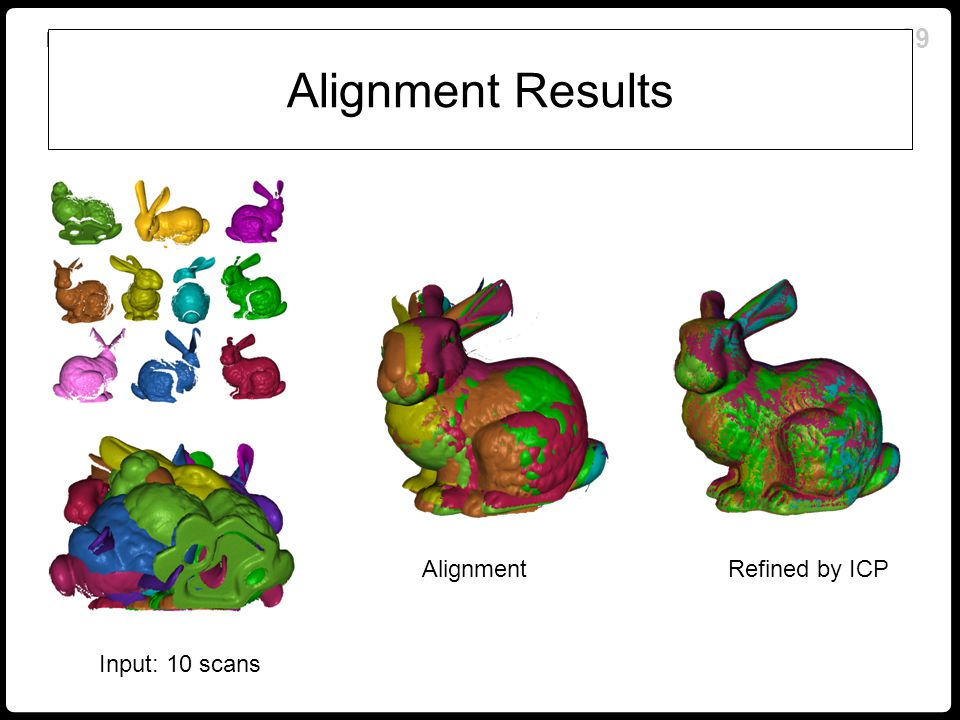
\includegraphics[width=300px]{results.jpg}
\end{center}
\end{figure}

%----------------------------------------------------------------------------------------
\end{document}
